\section{State-sharing multi-observer}\label{ch:ssmo}
In this chapter the state-sharing multi-observer (SSMO) will be discussed, aiming to reduce the required memory to store the CMO. The SSMO described in this chapter will provide the estimates as described in \autoref{subsec:state-estimates} and will employ the same selection procedure as described in \autoref{subsec:estimate-selection}.

\subsection{Constructing the state-estimates}
The SSMO follows the definition as in \cite{Chong2023MemoryAlgorithms}. Let
\begin{equation}\label{eqn:ssmo-observer}
    \begin{split}
        \dot{\hat{x}}_o &= \A_o\hat{x}_o - L_oC_ox + Bu -L_o(v_o + \tau_o), \quad \A_o=A+L_{o}C_{o} \\
    \end{split}
\end{equation}
be a set of observers that contains all $J$- and $P$-observers \eqref{eqn:cmo-single-J-observer}\eqref{eqn:cmo-single-P-observer}, such that $\mcO=\mcJ\bigcup\mcP$ and $o=1,2,\dots,|\mcO|$. All $L_o$ must be selected in such a way that all $\A_o$ share the same characteristic polynomial
\begin{equation}\label{eqn:ssmo-char-poly}
    \det(sI-\A) = p(s) = s^n + q_1s^{n-1} + \dots + q_{n-1}s + q_n
\end{equation}
and thus all have equal eigenvalues. Let us now define a matrix $\Tilde{L}_{o}$ such that $\Tilde{L}_oy=L_oy_o$. This can be achieved by padding $L_o$ with zero vectors $z \in \mathbb{R}^{n \times 1}$ \cite{Chong2023MemoryAlgorithms}. Let us now rewrite the observer \eqref{eqn:ssmo-observer} into the following form
\begin{equation}\label{eqn:ssmo-standard-system-form}
    \dot{\hat{x}}_o = \A_o\hat{x}_o + \B_o\eta_o, \quad
    \B_o =
    \begin{bmatrix}
        E & B & -\Tilde{L}_o \\
    \end{bmatrix}, \quad \eta_o =
    \begin{bmatrix}
        \phi(y) \\
        u \\
        y_o + v_o + \tau_o
    \end{bmatrix}.
\end{equation}

Let us now derive transformation matrices $T_o$ that transform all $\A_o$ and $\B_o$ as in \eqref{eqn:ssmo-standard-system-form} into controllable canonical form as in \cite[Sec. 4.3.2]{Hespanha2018LinearTheory}
\begin{equation}\label{eqn:controllable-canonical-form}
    \mathbf{A} =
    \begin{bmatrix}
        -q_1I_l & -q_2I_l & \cdots & -q_{n-1}I_l & -q_nI_l \\
        I_l & 0_l & \cdots & 0_l & 0_l \\
        0_l & I_l & \cdots & 0_l & 0_l \\
        \vdots & \vdots & \ddots & \vdots & \vdots \\
        0_l & 0_l & \cdots & I_l & 0_l \\
    \end{bmatrix}, \quad
    \mathbf{B} = 
    \begin{bmatrix}
        I_l \\ 0_l \\ \vdots \\ 0_l \\ 0_l \\
    \end{bmatrix}
\end{equation}
where $l=N$. The transformation matrices for each observer are,
\begin{equation}\label{eqn:ssmo-transformation}
    \begin{split}
        T_o &= R_pR_q\\
        R_p &=
        \begin{bmatrix}
            \B_o & \A_o\B_o & \A^{2}_o\B_o & \cdots & \A^{n-1}_o\B_o \\
        \end{bmatrix} \\
        R_q &=
        \begin{bmatrix}
            I_l & q_1I_l & q_2I_l & \cdots & q_{n-1}I_l \\
            0_l & I_l & q_1I_l & \cdots & q_{n-2}I_l \\
            \vdots & \ddots & \ddots & \ddots & \vdots \\
            0_l & \cdots & 0_l & I_l & q_1I_l \\
            0_l & \cdots & 0_l & 0_l & I_l \\
        \end{bmatrix}.
    \end{split}
\end{equation}
The calculation that shows that this transformation holds can be found in \autoref{ap:ssmo-transformation-matrix}. It should be noted that $\mathbf{A}$ and $\mathbf{B}$ are independent of $o$ and since all observers \eqref{eqn:ssmo-observer} share the same characteristic polynomial \eqref{eqn:ssmo-char-poly}, $\mathbf{A}$ and $\mathbf{B}$ are the same for all observers. This means that only one copy of the matrices needs to be stored and all state estimates $\hat{x}$ from the transformation matrices.

\subsection{Observer architecture}\label{subsec:ssmo-architecture}
Let us set the initial conditions of all state estimates to be equal, we will choose $0$ for simplicity. When all initial conditions are zero $z$ will also be the same for all state estimates, 
\begin{equation*}
    \dot{z} = \mathbf{A}z + \mathbf{B}\eta, \quad \eta = 
    \begin{bmatrix}
        u \\ y + v + \tau
    \end{bmatrix}.
\end{equation*}
We then transform $z$ into the original state estimates by

\begin{equation*}
    \tilde{x}_{SSMO} = \texttt{pm}(T,z,3),
\end{equation*}
where
\begin{center}
    % \begin{minipage}[t]{0.4\textwidth}
    %     \centering
    %     % first tikzpicture
    %     \begin{equation*}
    %         \begin{tikzpicture}[every node/.style={anchor=north east,fill=white,minimum width=1.2cm,minimum height=7mm}]
            
    %         % Define the displacement as a coordinate
    %         \coordinate (displacement) at (0.9,0.2);
        
    %         \matrix (mLP) [draw,matrix of math nodes]
    %             {
    %             \hat{x}_{\cP}^\mcJ \\
    %             };
        
    %         \matrix (dots2) [draw,matrix of math nodes] at ($(mLP.south west)+(displacement)$)
    %             {
    %             \dots \\
    %             };
        
    %         \matrix (mLp) [draw,matrix of math nodes] at ($(dots2.south west)+(displacement)$)
    %             {
    %             \hat{x}_{1}^\mcP \\
    %             };
        
    %         \matrix (mLJ) [draw,matrix of math nodes] at ($(mLp.south west)+(displacement)$)
    %             {
    %             \hat{x}_{\cJ}^\mcJ \\
    %             };
        
    %         \matrix (dots1) [draw,matrix of math nodes] at ($(mLJ.south west)+(displacement)$)
    %             {
    %             \dots \\
    %             };
        
    %         \matrix (mLj) [draw,matrix of math nodes] at ($(dots1.south west)+(displacement)$)
    %             {
    %             \hat{x}_1^\mcJ \\
    %             };
            
    %         \draw[dashed](mLj.north east)--(mLP.north east);
    %         \draw[dashed](mLj.north west)--(mLP.north west);
    %         \draw[dashed](mLj.south east)--(mLP.south east);
            
    %         \node at ($(-4,-1.8)$) {$\hat{x}_{SSMO}=$};
            
    %         \end{tikzpicture}
    %     \end{equation*}
    % \end{minipage}
    \begin{minipage}[t]{0.4\textwidth}
    \centering
    % Second tikzpicture
        \begin{equation}\label{eqn:T-ssmo}
            \begin{tikzpicture}[every node/.style={anchor=north east,fill=white,minimum width=2cm,minimum height=7mm}]
            
            % Define the displacement as a coordinate
            \coordinate (displacement) at (1.7,0.2);
        
            \matrix (mLP) [draw,matrix of math nodes]
                {
                T^\mcP_{N_P} \\
                };
        
            \matrix (dots2) [draw,matrix of math nodes] at ($(mLP.south west)+(displacement)$)
                {
                \dots \\
                };
        
            \matrix (mLp) [draw,matrix of math nodes] at ($(dots2.south west)+(displacement)$)
                {
                T^\mcP_{1} \\
                };
        
            \matrix (mLJ) [draw,matrix of math nodes] at ($(mLp.south west)+(displacement)$)
                {
                T^\mcJ_{N_J} \\
                };
        
            \matrix (dots1) [draw,matrix of math nodes] at ($(mLJ.south west)+(displacement)$)
                {
                \dots \\
                };
        
            \matrix (mLj) [draw,matrix of math nodes] at ($(dots1.south west)+(displacement)$)
                {
                T^\mcJ_1 \\
                };

            
            \draw[dashed](mLj.north east)--(mLP.north east);
            \draw[dashed](mLj.north west)--(mLP.north west);
            \draw[dashed](mLj.south east)--(mLP.south east);
            
            \node at ($(-4,-1.8)$) {$T=$};
            
            \end{tikzpicture}
        \end{equation}
    \end{minipage}
\end{center}
The structure of the storage matrix $\tilde{x}_{SSMO}$ is the same as $\tilde{x}_{3D}$ in \eqref{eqn:A-tilde-3D}. The selection of the final estimate follows the same procedure as described in Section \ref{subsec:estimate-selection}.

\begin{table}[h]
    \centering
    \begin{tabular}{|c|c|c|}
        \toprule
       Matrix  & Dimensions & Number of elements \\ \midrule
       $\Tilde{x}_{SSMO}$  & $ n_x \times 1 \times N_S$ & $n_xN_S$ \\
       $\mathbf{A}$ & $n_xN_O \times n_xN_O$ & $n_x^2N_O^2$ \\ 
       $\mathbf{B}$ & $n_xN_O \times n_x$ & $n_x^2N_O$ \\
       $T$ & $n_x \times n_xN_O \times N_S$ & $n_x^2N_ON_S$ \\
       \bottomrule
    \end{tabular}
    \caption{SSMO system matrix dimensions}
    \label{tab:SSMO-dimensions}
\end{table}

\subsection{Size comparison}
Let us now compare the sizes of the 2D-CMO, 3D-CMO and SSMO as presented in Tables \ref{tab:2D-CMO-dimensions}, \ref{tab:3D-CMO-dimensions} and \ref{tab:SSMO-dimensions} respectively. First, the total number of elements for each MO is derived from the matrices that are needed to construct it. 
\begin{table}[h]
    \centering
    \begin{tabular}{|c|c|}
        \toprule
        Multi-Observer & Total number of Elements \\
        \midrule
        2D-CMO & $n_xN_S + n_x^2N_S^2 + 2n_uN_S$ \\
        3D-CMO & $n_xN_S + 2n_x^2N_S$ \\
        SSMO   & $n_xN_S + n_x^2N_O^2 + n_x^2N_O + n_x^2N_ON_S$ \\
        \bottomrule
    \end{tabular}
    \caption{Total number of elements in each MO implementation}
    \label{tab:my_label}
\end{table}

We now use the for $N_S$ as in equation \eqref{eqn:NS-approximation} to compare number of Gigabytes required to store the MO. This value is derived from the number of elements, each element requires 8 bytes to be stored in for example a python float or a Matlab double. The comparison is made for different combinations of the number of state variables $n_x$ and number of total system outputs $N_O$. Both of these values are ranged from $1$ to $50$ and the storage size for each combination is compared.

Figure \ref{fig:MO-storage}, where the colour indicates the total size of the MO, shows the result of this comparison. The 2D CMO performs very poorly, as to be expected due to the $N_S^2$ term appearing in it's $A$ matrix (see \autoref{tab:2D-CMO-dimensions}). The 3D CMO and the SSMO perform similarly. The size of all MOs increases much more with an increasing $N_O$ as compared to a growing $n_x$, which is not strange considering $N_O$ influences the number of combinations that need to be made from all sensors.


\begin{figure}[H]
    \centering
    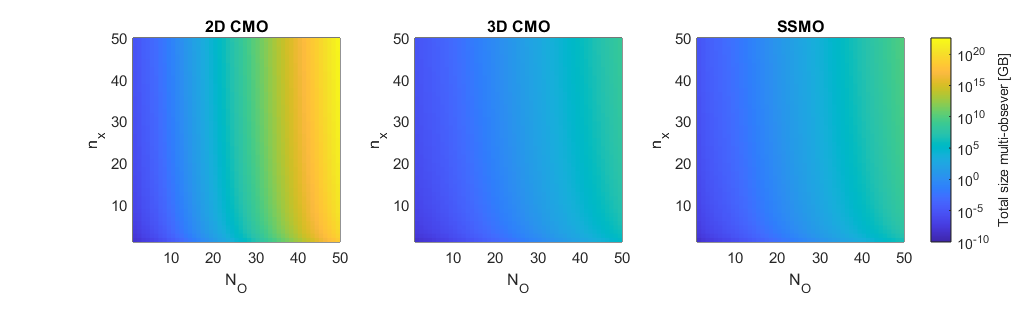
\includegraphics[width=\linewidth]{report/Figures/sizeComparison60.png}
    \caption{Storage requirements for different MOs}
    \label{fig:MO-storage}
\end{figure}


In Figure \ref{fig:ssmo-vs-3dcmo} the SSMO size is divided by the 3D CMO size, the plot shows the ratio between the two MOs. The figure clearly shows that the 3D CMO uses less memory than the SSMO under every circumstance. The difference becomes more pronounced for larger values of $N_O$. This can be attributed to the size of the $T$ matrix in Equation \ref{eqn:T-ssmo}, where its size $n_x^2N_ON_S$ can be viewed as $n_x^3N_S$ on the diagonal in Figure \ref{fig:ssmo-vs-3dcmo}.

\begin{figure}[H]
    \centering
    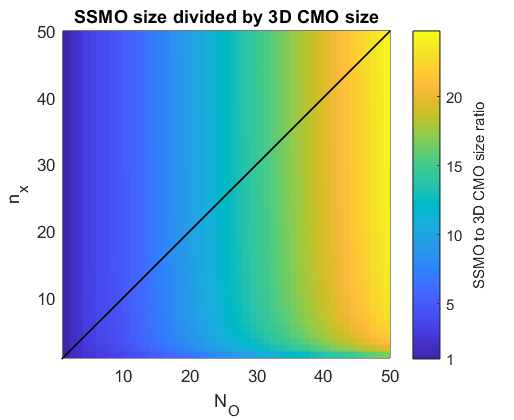
\includegraphics[width=0.4\linewidth]{report/Figures/ssmo_vs_3dcmo.png}
    \caption{Ratio between the required memory for an SSMO and 3D CMO respectively}
    \label{fig:ssmo-vs-3dcmo}
\end{figure}

It should also be noted that none of the MOs can be implemented in scenarios with a large $N_O$, since the required memory is enormous. Even the super computer Frontier with 9.6 Petabytes ($10^6$ Gigabytes) of random access memory would not be able to run such an MO \cite{2024FrontierDocumentation}.